\section{Real-data case: recorded vehicle trajectories}
\label{sec:real-case}

\subsection{Observed data are not known true jerk}
The Federal Highway Administration's NGSIM US-101 and
I-80 trajectories supply camera-derived longitudinal position,
not independent noise-free physical position or jerk.
For an initial visualization we retain the five
prespecified US-101 track segments from the original
case study, comprising 15 overlapping training/forecast
origins and only two distinct integer vehicle IDs.
The more informative recorded-position validation uses
$200$ preselected NGSIM episodes ($100$ from each site),
each with 80 past 0.1-s observations and 5, 10 and
20 future frames withheld. The source and selection
rules were frozen before model comparisons.
These episodes correspond to 113 distinct
(site, integer vehicle ID) pairs and five
coarse recording-time blocks; repetitions
of an integer identifier need not be the same
physical driver. Our pooled error summaries are
descriptive and do not justify treating 200
episodes as independent population draws.

\begin{figure*}[t]
\centering
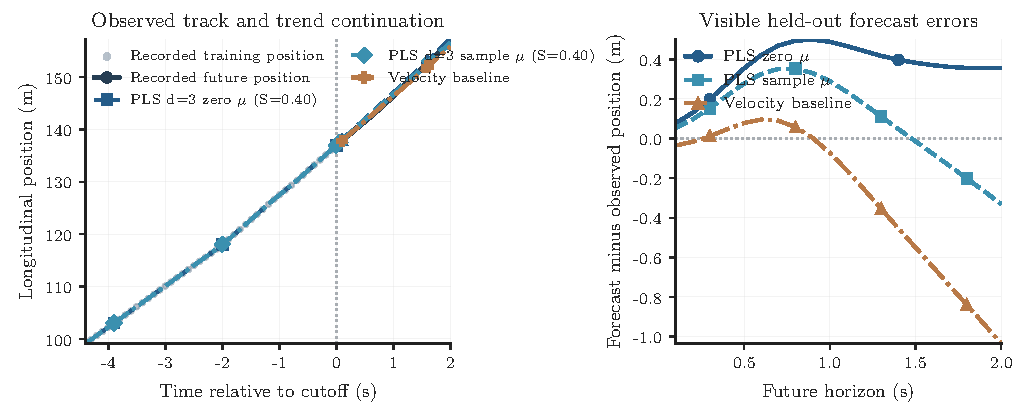
\includegraphics[width=\textwidth]{figures/heldout_forecast.pdf}
\caption{Predeclared chronological US-101 illustration:
the measured historical segment, withheld future
recorded positions, fitted third-order PLS trends
with zero and training-derived reference means,
and their historical-trend extrapolations.
No future observation enters historical fitting
or smoothing-parameter selection. This pilot
figure is not drawn from the larger 200-episode
sample to claim an additional independent test.}
\label{fig:forecast}
\end{figure*}

\begin{figure*}[t]
\centering
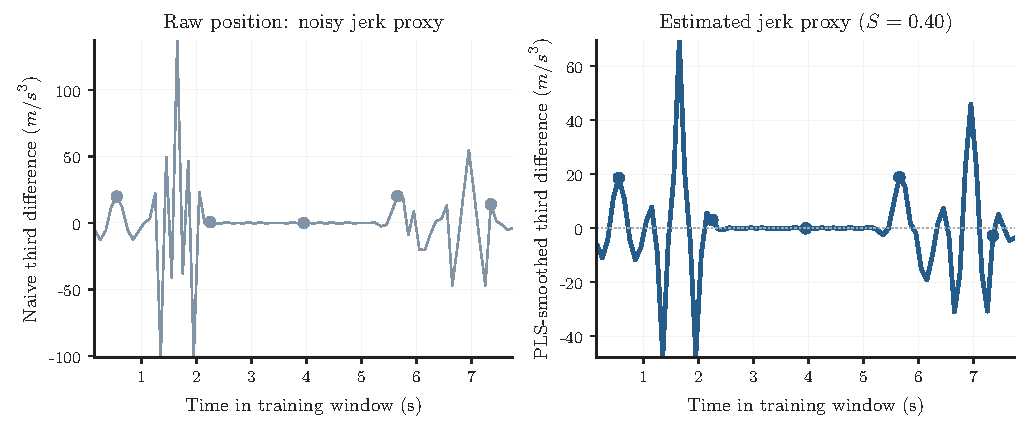
\includegraphics[width=\textwidth]{figures/jerk_comparison.pdf}
\caption{Raw and PLS-regularized \emph{proxies}
for third differences of the same measured
US-101 position segment, scaled by
$(0.1\,\mathrm{s})^3$ to have jerk units.
The panels use different axes. A smoother
curve is not proof of physical jerk accuracy:
this real recorded trajectory has no
independently measured true jerk.}
\label{fig:jerk}
\end{figure*}

\subsection{Matched PLS versus spectral SVD and physical baselines}
The SVD comparison is based on the same original
$200$ recorded episodes and reuses archived,
training-selected global cubic OLS references
and continuous Gaussian profile-ML penalties.
SVD-GCV chooses its rank using historical
positions only under the conditional plug-in
criterion in Eq.~\eqref{eq:tsvd-conditional-gcv}.
The matched-rank SVD equates \emph{nominal
fixed-reference} effective complexity with PLS;
it does not exactly match the full data-dependent
estimator's degrees of freedom. The same
three-point continuation \emph{algorithm}
in Eq.~\eqref{eq:d3-recurrence} is applied
to each historical fit. Its reference
$\mu$ is the common training-derived
cubic-OLS value for PLS and TSVD, but zero
for spline and Savitzky--Golay fits.
Thus the boundary rule is shared, not every
model assumption or third-difference
reference. The comparison is not a
benchmark of Cholesky versus SVD run time.

\begin{table*}[t]
\centering
\caption{Future \emph{recorded-position}
RMSE (m) averaged over frames 1 through
$H=5,10,20$ in each of $200$ selected NGSIM
episodes, with chronological 80-point training
windows. Values are \emph{cumulative-window}
errors (Eq.~\eqref{eq:forecast-window-rmse}),
not terminal-frame errors. The first five rows
use the common three-point constant-third-
difference continuation; the final
GCV spline row uses its \emph{own}
quadratic Taylor continuation and is
therefore an end-to-end method comparison,
not an identical boundary-rule ablation.
No independent true jerk is available.}
\label{tab:real-svd}
\begin{tabular}{lccc}
\toprule
Historical smoother + continuation & $H=5$ & $H=10$ & $H=20$\\
\midrule
PLS, cubic OLS reference + profile ML
& 0.1434 & 0.5144 & 1.8829\\
SVD cutoff, matched complexity
& 0.1423 & 0.5118 & 1.8787\\
SVD cutoff, training-only GCV rank
& 0.1512 & 0.5337 & 1.9339\\
Natural cubic smoothing spline, GCV
& 0.1393 & 0.4946 & 1.7965\\
Savitzky--Golay (21,3)
& 0.3464 & 0.8188 & 2.2822\\
\midrule
GCV natural cubic spline + quadratic Taylor
& \textbf{0.1354} & \textbf{0.3480} & \textbf{0.8787}\\
\bottomrule
\end{tabular}
\end{table*}

\begin{figure*}[t]
\centering
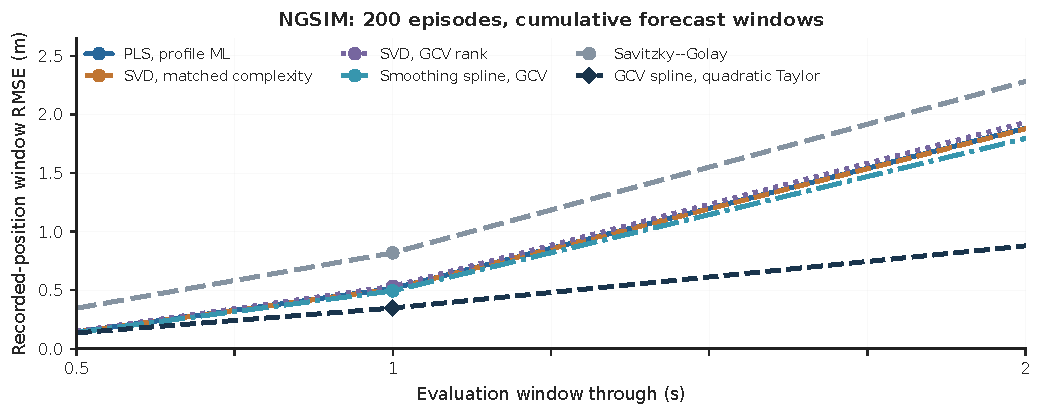
\includegraphics[width=\textwidth]{figures/exp008_real_forecast_benchmarks.pdf}
\caption{Recorded-future longitudinal position
cumulative-window RMSE across $200$ real NGSIM
episodes and three evaluation windows (0.5, 1 and 2\,s). Five historical smoothers
share the same last-three-point continuation,
with the independently selected GCV cubic
spline and quadratic Taylor forecast
shown as an additional dashed-line
\emph{end-to-end} benchmark. The
recorded future is the only observable
target; no latent position or true jerk
appears in these errors.}
\label{fig:real-svd}
\end{figure*}

In the new matched-complexity comparison,
PLS and hard-truncated SVD produce very
similar pooled first-second recorded-position
window RMSE ($0.5144$ and $0.5118$\,m). This
real-data result does \emph{not} establish
superiority of PLS over SVD on forecasting,
despite its stronger known-jerk reconstruction
performance in Section~\ref{sec:synthetic-case}.
The GCV cubic smoothing spline with quadratic
Taylor extrapolation achieves smaller pooled
recorded-position window RMSE at each horizon.
The comparison changes both the historical smoother
and its continuation; it cannot attribute the
entire difference to spline smoothing alone.
An alternative continuation of the
\emph{same fitted historical trend} can
therefore matter as much as the smoother.

\subsection{Original historical illustration and forecast horizons}
The smaller original exploratory study
compared PLS under several difference orders,
regularization criteria and $\mu$ choices,
then examined a last-three-point
$d=3$ continuation. Those original
numerical tables and all four-order
criterion heatmaps are retained in the
research archive rather than treated
as the main evidence of physical superiority.

\begin{figure*}[t]
\centering
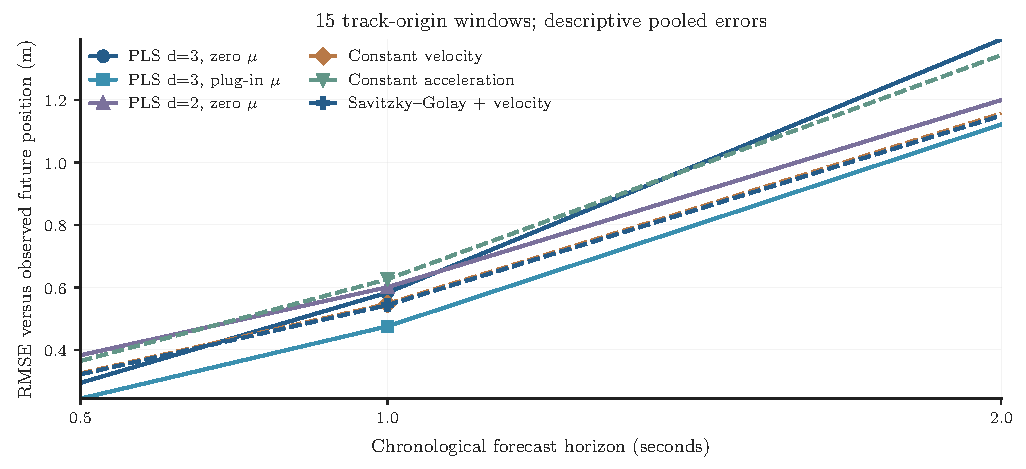
\includegraphics[width=\textwidth]{figures/forecast_horizons.pdf}
\caption{Original exploratory chronological
comparison over 15 overlapping forecast
origins from five US-101 track segments,
including PLS and conventional
constant-velocity, constant-acceleration
and Savitzky--Golay baselines.
The plotted horizons use measured future
positions, not known underlying truth.
This smaller sample is not independent
of the historical case-study provenance,
nor representative of the larger
200-episode follow-up.}
\label{fig:horizons}
\end{figure*}

In the original 15-origin comparison,
PLS with zero reference and the
three-point $d=3$ recurrence attained
$0.0745$\,m pooled observed-position
RMSE at $0.5$\,s, whereas the
GCV spline's quadratic continuation
attained $0.1233$\,m. At $2$\,s,
the spline attained $0.8085$\,m
versus $1.2998$\,m for that PLS
recurrence. These rankings are
\emph{exploratory}; the larger
200-episode study demonstrates how
small-sample method comparisons can
change with different recorded cases.
